\documentclass[10pt,a4paper]{article}
\author{Elijah Andrews}
\usepackage[latin1]{inputenc}
\usepackage{amsmath}
\usepackage{amsfonts}
\usepackage{amssymb}
\usepackage[labelfont=bf]{caption}
\usepackage{graphicx}
\usepackage{csvsimple}
\usepackage[left=2cm,right=2cm,top=2cm,bottom=2cm]{geometry}
\usepackage{fancyhdr}
\usepackage[section]{placeins}
 
\pagestyle{fancy}
\fancyhf{}
\fancyhead[LE,RO]{Elijah Andrews}
\fancyhead[RE,LO]{Wing Aerodynamics Coursework}
\fancyfoot[CE,CO]{\leftmark}
\fancyfoot[LE,RO]{\thepage}

\makeatletter
\AtBeginDocument{%
  \expandafter\renewcommand\expandafter\subsection\expandafter{%
    \expandafter\@fb@secFB\subsection
  }%
}
\makeatother

\makeatletter
\AtBeginDocument{%
  \expandafter\renewcommand\expandafter\subsubsection\expandafter{%
    \expandafter\@fb@secFB\subsubsection
  }%
}
\makeatother

\makeatletter
\csvset{
  autotabularcenter/.style={
    file=#1,
    after head=\csv@pretable\begin{tabular}{|*{\csv@columncount}{c|}}\csv@tablehead,
    table head=\hline\csvlinetotablerow\\\hline,
    late after line=\\,
    table foot=\\\hline,
    late after last line=\csv@tablefoot\end{tabular}\csv@posttable,
    command=\csvlinetotablerow},
  autobooktabularcenter/.style={
    file=#1,
    after head=\csv@pretable\begin{tabular}{*{\csv@columncount}{c}}\csv@tablehead,
    table head=\toprule\csvlinetotablerow\\\midrule,
    late after line=\\,
    table foot=\\\bottomrule,
    late after last line=\csv@tablefoot\end{tabular}\csv@posttable,
    command=\csvlinetotablerow},
}
\makeatother
\newcommand{\csvautotabularcenter}[2][]{\csvloop{autotabularcenter={#2},#1}}
\newcommand{\csvautobooktabularcenter}[2][]{\csvloop{autobooktabularcenter={#2},#1}}

\usepackage{siunitx,array,booktabs}
\begin{document}
\section{Part I}
\subsection{Aerofoil Generation}
\begin{figure}[!htb]
\centering
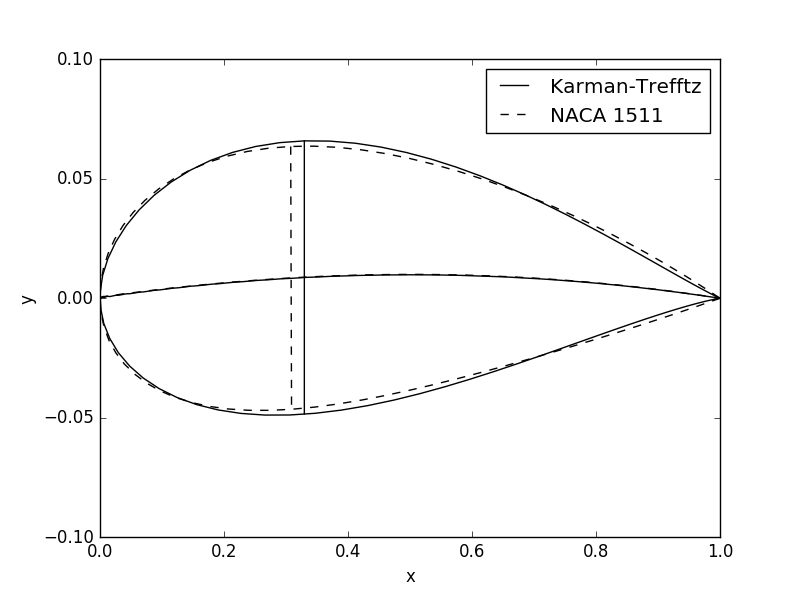
\includegraphics[scale=0.75]{Figures/ktreff_naca_comparison.png}
\caption{A comparison between a Karman-Trefftz aerofoil and its closest NACA aerofoil.}
\label{fig:ktreff_naca_comparison}
\end{figure}
\subsection{Parameter Variation}
\begin{figure}[!htb]
\centering
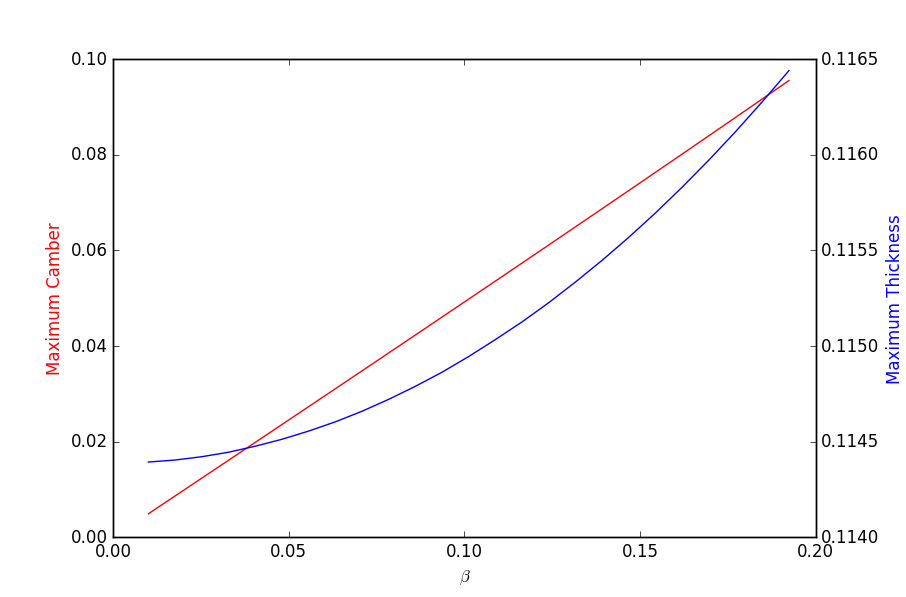
\includegraphics[scale=0.6]{Figures/beta_variation.png}
\caption{How maximum thickness and maximum camber change with $\beta$.}
\label{fig:beta_variation}
\end{figure}
\begin{figure}[!htb]
\centering
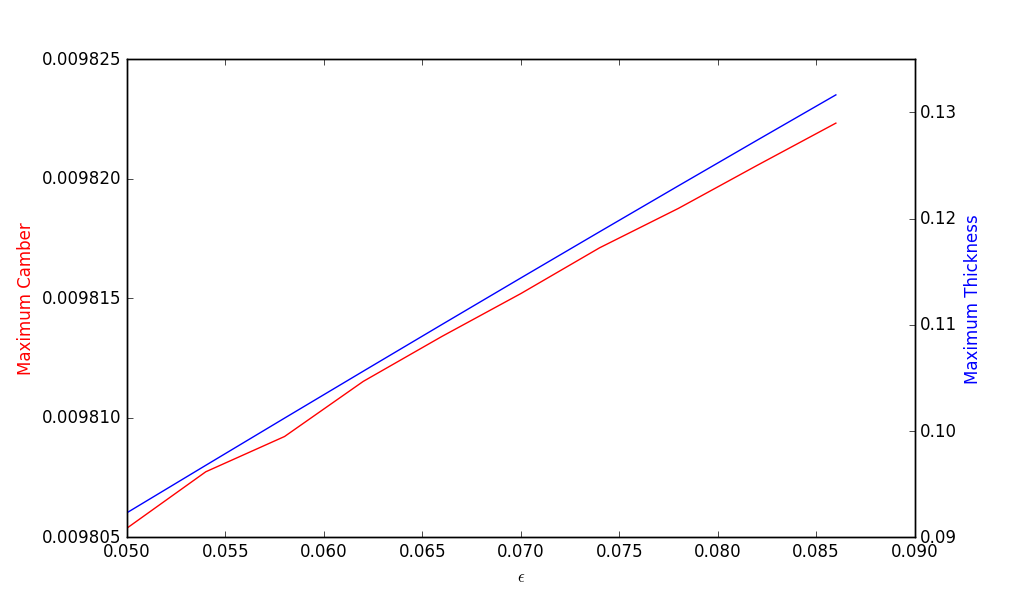
\includegraphics[scale=0.6]{Figures/epsilon_variation.png}
\caption{How maximum thickness and maximum camber change with $\epsilon$.}
\label{fig:epsilon_variation}
\end{figure}
\section{Part II}
\subsection{Doublet Panel Method Accuracy}
\begin{figure}[!htb]
\centering
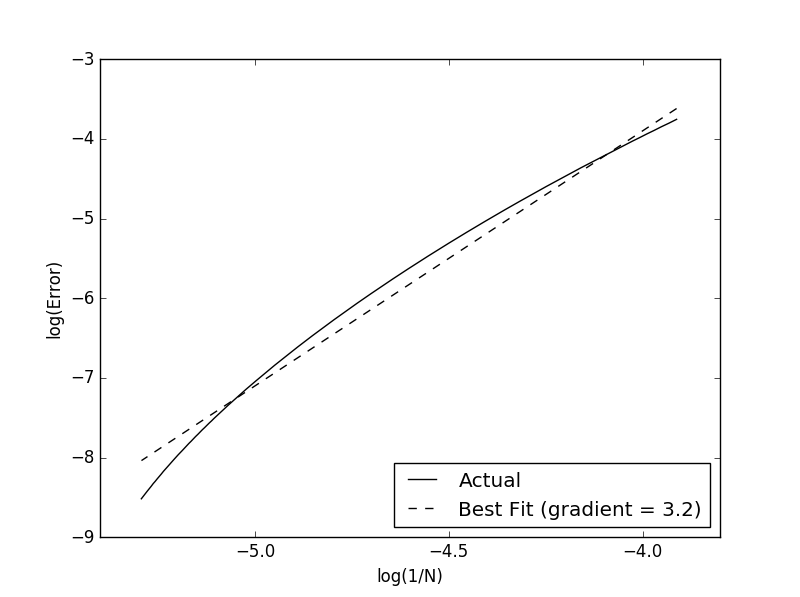
\includegraphics[scale=0.75]{Figures/accuracy.png}
\caption{Accuracy of the Doublet Panel Method.}
\label{fig:accuracy}
\end{figure}
\subsection{NACA and Karman-Trefftz Performance Comparison}
\subsubsection{Lift, Drag, and Stall Characteristics}
\begin{figure}[!htb]
\centering
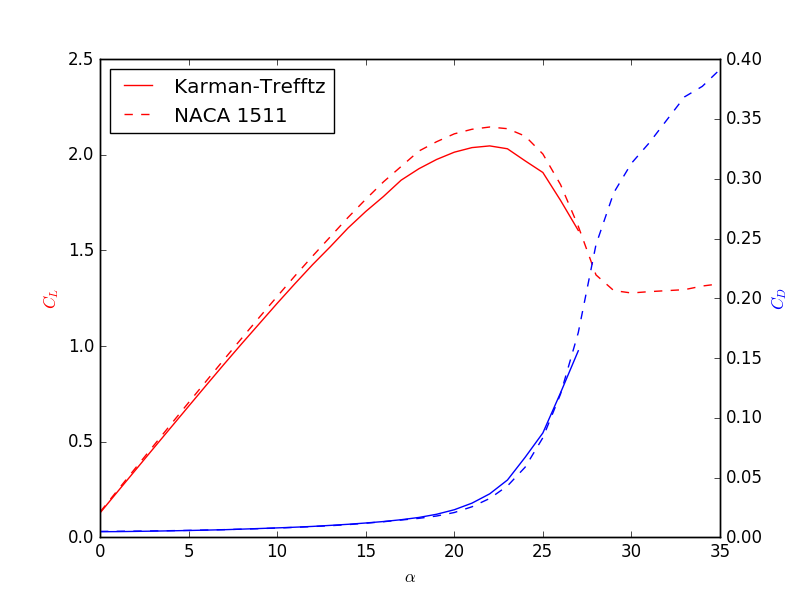
\includegraphics[scale=0.75]{Figures/polar_characteristics.png}
\caption{Lift, drag, and stall characteristics for the Karman-Trefftz and NACA 1511 aerofoils.}
\label{fig:characteristics}
\end{figure}
\subsubsection{Transition Position}
\begin{figure}[!htb]
\centering
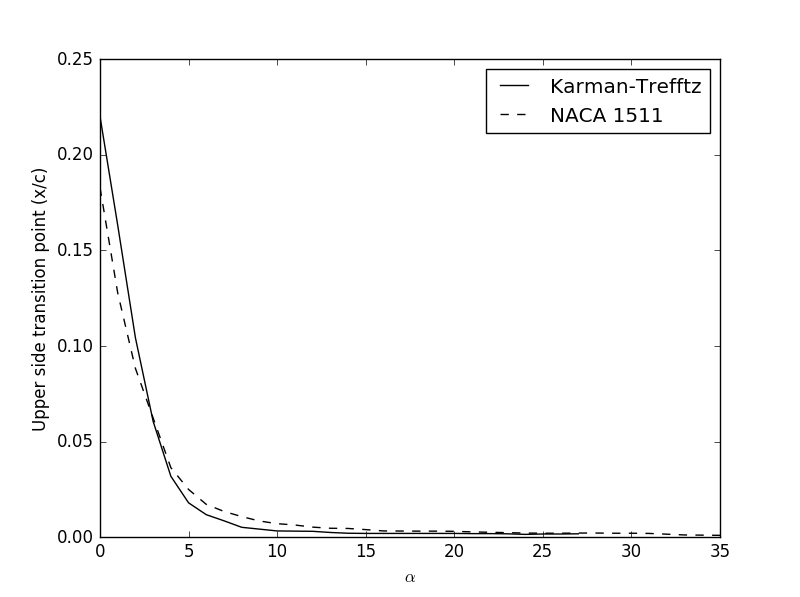
\includegraphics[scale=0.75]{Figures/transition_comparison.png}
\caption{Comparison of transition point between NACA 1511 and Karman-Trefftz aerofoils.}
\label{fig:transition_comparison}
\end{figure}
\subsubsection{Separation Position}
\begin{figure}[!htb]
\centering
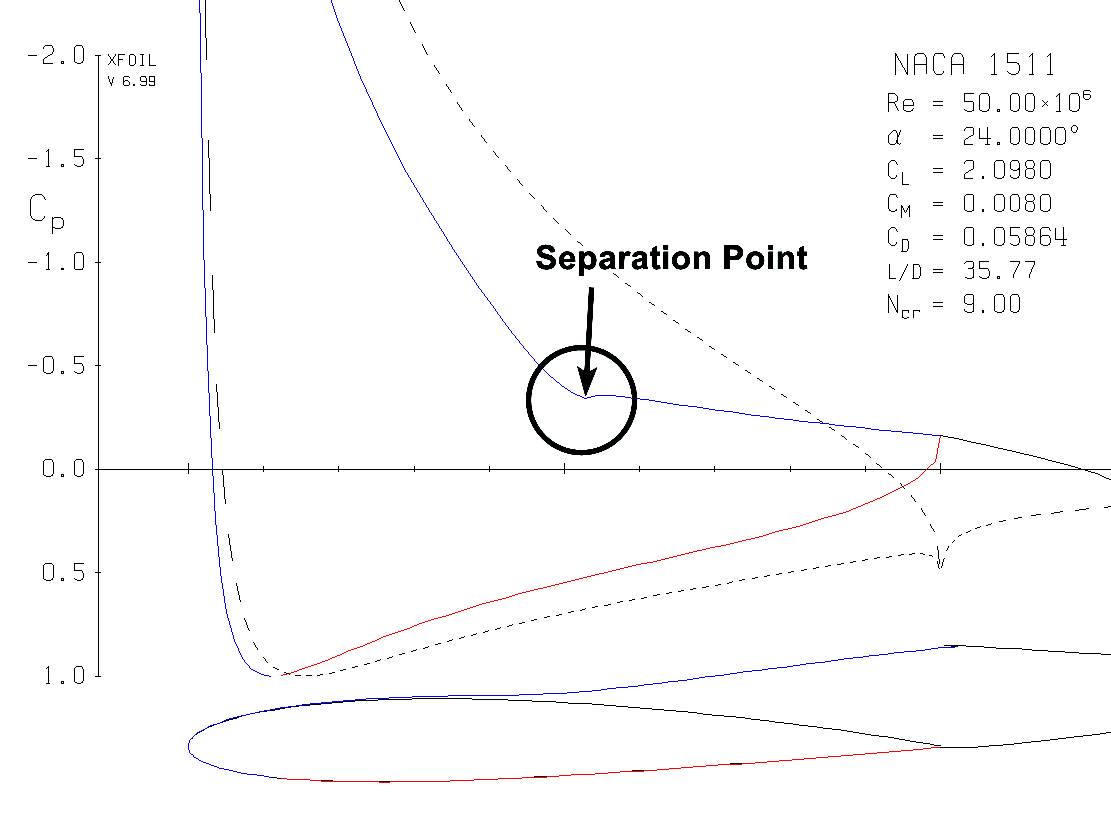
\includegraphics[scale=0.5]{Figures/separation_point.png}
\caption{The definition of the separation point used in this coursework.}
\label{fig:separation_point}
\end{figure}
\begin{figure}[!htb]
\centering
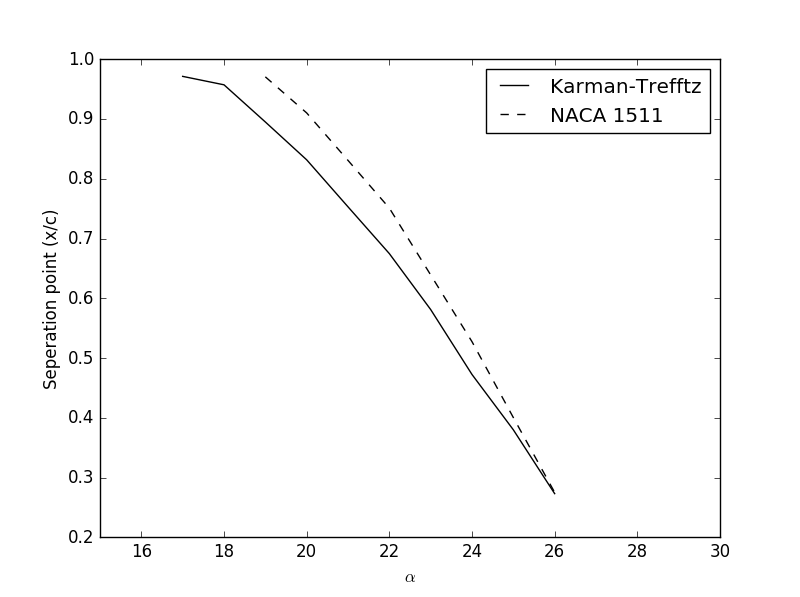
\includegraphics[scale=0.75]{Figures/separation_comparison.png}
\caption{Comparison of separation point between NACA 1511 and Karman-Trefftz aerofoils.}
\label{fig:separation_comparison}
\end{figure}
\end{document}
